\documentclass[a4paper]{article}
\usepackage[utf8]{inputenc}
\usepackage[english]{babel}
\usepackage{amsmath} % per ambienti tipo cases
\usepackage{mathtools}
\usepackage{siunitx}
\usepackage{graphicx} % per includere figure
%\usepackage{subfigure}
\usepackage{booktabs} % per le tabelle
\usepackage{caption}
\usepackage{fancyhdr}
\usepackage{hyperref}
\usepackage[section]{placeins}
\usepackage{microtype}
\usepackage{caption}
\usepackage{subcaption}
\usepackage{verbatim} %multiline comments
\usepackage[backend=biber, style=numeric, safeinputenc, sorting=none]{biblatex}
\addbibresource{source.bib}
\captionsetup[subfigure]{labelfont=rm}


%opening
\title{}
\author{}

\pagestyle{fancy}
\lhead{Musical Acoustics}
\chead{Homework 2}
\rhead{10743504, 10751919}
\newcommand{\Rarrow}{\mbox{\Large$\Rightarrow$}}

\begin{document}

\begin{titlepage}	
	\newcommand{\HRule}{\rule{\linewidth}{0.5mm}} % Defines a new command for horizontal lines, change thickness here
	
	\center % Centre everything on the page
	
	%------------------------------------------------
	%	Headings
	%------------------------------------------------
	
	
\includegraphics[width=.4\textwidth]{Logo_Politecnico_Milano.png}\\[0.4cm]
	\textsc{\LARGE}\\[0.3cm] % Main heading such as the name of your university/college
	
	\textsc{\large MSc. Music and Acoustic Engineering}\\[1cm] % Minor heading such as course title
	
	\textsc{\Large Musical Acoustics - A.Y. 2020/2021}\\[0.5cm] % Major heading such as course name
	
	%------------------------------------------------
	%	Title
	%------------------------------------------------
	
	\HRule\\[0.4cm]
	
	{\huge\bfseries Homework 2 - Soundboard modeling and string coupling}\\[0.4cm] % Title of your document
	
	\HRule\\[1.5cm]
	
	
	
	{\large\textit{Authors' IDs:}}\\
	10743504, 10751919, % Your name
	%\\ \textsc{Gruppo 11}
	
	%------------------------------------------------
	%	Date
	%------------------------------------------------
	
	\vfill\vfill\vfill % Position the date 3/4 down the remaining page
	
	{\large\today} % Date, change the \today to a set date if you want to be precise
	
	%------------------------------------------------
	%	Logo
	%------------------------------------------------
	
	\vfill\vfill
	%\includegraphics[width=0.2\textwidth]{Politecnico_di_Milano.eps}\\[1cm] % Include a department/university logo - this will require the graphicx package
	
	%----------------------------------------------------------------------------------------
	
	\vfill % Push the date up 1/4 of the remaining page
	
	
\end{titlepage}

%\begin{abstract}
%\end{abstract}

\section{Lowest modal frequencies}
\subsection{Supported edges}
The most straightforward case is that of supported edges, as it is the only one for which we have an analytical expression of the eigenshapes and eigenfrequencies. As we have seen in class, the modal shapes are:
$$ Z_{mn}(x, y) = A\sin\left( 	\frac{(m+1)\pi x}{L_x} \right) \sin\left( 	\frac{(n+1)\pi x}{L_y} \right), \quad m,n = 0, 1, \dots$$
where in our case $L_x = \SI{1}{\meter}$ and $L_y = \SI{1.4}{\meter}$.
The related eigenfrequencies are:
$$ f_{mn} = 0.453c_L h \left[\frac{(m+1)^2}{L_x^2} + \frac{(n+1)^2}{L_y^2}\right] $$
where $c_L$ is the longitudinal wave velocity and $h = \SI{3}{\milli\meter}$ is the plate thickness. The values of the lowest five modes for these boundary conditions are reported in Tab. \ref{tab:ssfreq}.

\begin{table}[h]
	\centering
	$\begin{array}{l|lllll}
		\toprule
		\text{Modes} & (0,0) & (0,1) & (1,0) & (0,2) & (1,1) \\
		\hline
		\text{Freqs[Hz]} & 11.18 & 22.51 & 33.39 & 41.40 & 44.72\\
		\bottomrule
	\end{array}$
	\caption{Modal frequencies for the lowest five modes with supported edges.}
	\label{tab:ssfreq}
\end{table}

\subsection{Free edges}

Considering boundary conditions different from those of the previous case complicates the problem considerably. However, during class we have covered the eigenfrequencies of a square plate with free edges: in particular, we have been given the ratios of the frequencies of the first 10 modes with that of the first mode $f_{11}$ for a square plate with Poisson's ratio $\nu = 0.3$. Since the Poisson's ratio of our plate is close to this value and its aspect ratio is quite close to 1, a first approach is to simply compute the natural frequencies as if the plate were square, with the lowest frequency written as:
$$ f_{11} = \frac{hc_L}{L_x L_y} \sqrt{\frac{1-\nu}{2}} $$

The modal frequencies computed with this approximation are reported in Tab. \ref{tab:sqffreq}. Notice how the last two modes are degenerate: this is of course true for a square plate, but we would expect to see two different frequencies for these two modes in our rectangular plate.


\begin{table}[h]
	\centering
	$\begin{array}{l|lllll}
		\toprule
		\text{Modes} & (1,1) & (2,0) - (0,2) & (2,0) + (0,2) & (2,1) & (1,2) \\
		\hline
		\text{Freqs[Hz]} & 6.47 &  9.83 & 
		12.55 &  17.53  & 17.53 \\
		\bottomrule
	\end{array}$
	\caption{Modal frequencies for the lowest five modes with free edges, in the square plate approximation.}
	\label{tab:sqffreq}
\end{table}

If we wanted a more refined model, of course, approximate solutions for this problem have been known since Lord Rayleigh; in \cite{leissa} we find a review of the main results of these kind of solutions developed throughout the 20th century. We report in Tab. \ref{tab:ffreq} the lowest five modal frequencies for a plate with aspect ratio $1.5$ and $\nu = 1/6 $.

\begin{table}[h]
	\centering
	$\begin{array}{l|lllll}
		\toprule
		\text{Modes} & (1,1) & (0,2) & (1,2) & (2,0) & (3,0) \\
		\hline
		\text{Freqs[Hz]} & 7.07 &  7.09 & 
		15.87 &  15.96  & 19.55	\\
		\bottomrule
	\end{array}$
	\caption{Modal frequencies for the lowest five modes for a free plate with $\nu = 1/6$ and $a/b = 2/3$ from \cite{leissa}.}
	\label{tab:ffreq}
\end{table}

For this case and that of clamped edges we also performed numerical simulations in COMSOL. We report the results of these simulations in the appendix; however, we point out here that, despite the significant difference in the value of $\nu$ for the previous table from that of our plate, the results of the simulations are closer to these values than to those from the square plate approximation.

\subsection{Clamped edges}

For clamped edges, again, we don't have an analytical solution. We can use the same approach here and compute the eigenfrequencies as if the plate were square. The fundamental frequency can be written this time as $f_{00} = 1.654c_l h / L_xL_y$. The results are reported in Tab. \ref{tab:sqcfreq}. Of course here too we find two degenerate modes, to which the same considerations as before apply.

\begin{table}[h]
	\centering
	$\begin{array}{l|lllll}
		\toprule
		\text{Modes} & (0,0) & (1,0) & (0,1) & (1,1) & (2,0) - (0,2) \\
		\hline
		\text{Freqs[Hz]} & 19.3 &  39.39 & 
		39.39 &  58.11  & 70.66	\\
		\bottomrule
	\end{array}$
	\caption{Modal frequencies for the lowest five modes of the clamped plate in the square plate approximation.}
	\label{tab:sqcfreq}
\end{table}

In \cite{leissa}, more accurate values for the eigenfrequencies of a clamped plate can be found for a variety of aspect ratios. The value of the aspect ratio closest to that of our plate is 0.72; the corresponding lowest five modal frequencies are reported in Tab. \ref{tab:cfreq}.

\begin{table}[h]
	\centering
	$\begin{array}{l|lllll}
		\toprule
		\text{Freqs[Hz]} & 21.06 & 34.33  & 
		50.31 &  56.36  & 62.57\\
		\bottomrule
	\end{array}$
	\caption{Modal frequencies for the lowest five modes of a clamped plate with aspect ratio 0.72.}
	\label{tab:cfreq}
\end{table}

%\cite{leissa}
%\cite{fletchross}
%\cite{chker}

Overall, we can gather that the boundary conditions have an impact on the eigenfrequencies that appears to be more significant than changes in the aspect ratio or the physical parameters.

\section{Boundary conditions and modal density}

The frequency separations for the three cases discussed in the previous section can be seen in Tab. \ref{tab:sep}. 
Moreover, we can compute a rough estimate of the modal density by dividing the number of modes (5) by the frequency separation between the highest and lowest modes. The results are $0.38~\si{\hertz^{-1}}$ for the free edges, $0.15~\si{\hertz^{-1}}$ for the supported edges and $0.12~\si{\hertz^{-1}}$ for the clamped edges.

\begin{table}[h]
		\centering
		$\begin{array}{l|llll}
			\toprule
			 & \delta_{21} & \delta_{32} & \delta_{43} & \delta_{54}\\
			\midrule
			\text{Free edges} & \SI{0.03}{\hertz} & \SI{9.24}{\hertz} & \SI{0.10}{\hertz}  & \SI{3.78}{\hertz}\\
			\text{Supported edges} & \SI{11.33}{\hertz}  & \SI{10.88}{\hertz}  &  \SI{8.01}{\hertz}  &  \SI{3.32}{\hertz}\\
			\text{Clamped edges} & \SI{13.27}{\hertz} &  \SI{15.98}{\hertz}  &  \SI{6.05}{\hertz}  &  \SI{6.22}{\hertz}\\
			\bottomrule
		\end{array}$
		\caption{Frequency separations between the lowest modes.}
		\label{tab:sep}
\end{table}

Notice how increasing the restraint on the edges of the plate tends to increase the separations between the eigenfrequencies and, conversely, decrease the modal density. This is a consequence of the increase in stiffness that comes from these additional restraints, which means an increase in the fundamental frequency.


\section{Effect on non-linearities on the natural frequencies}

\begin{figure}[h]
	\centering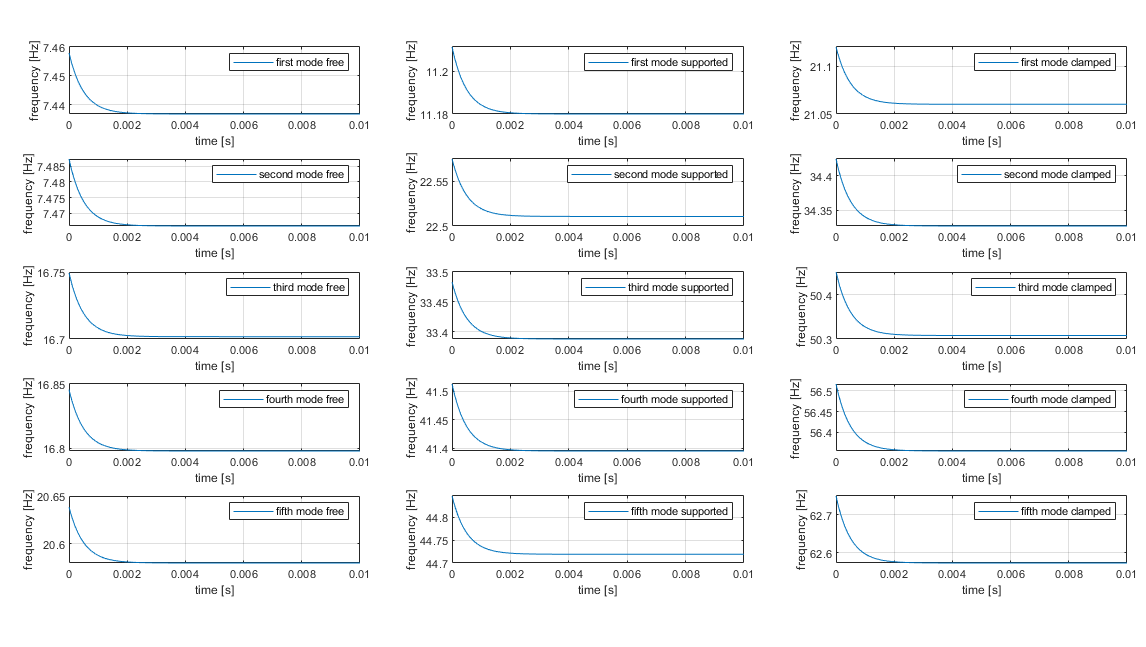
\includegraphics[width=0.95\textwidth]{point_3.png}
	\caption{Time plots of the frequencies of the natural modes with decay time $1$ ms. From left to right: free edges, supported edges, clamped edges.}
	\label{fig:dec}
\end{figure}

As we know from the study of the vibration of shells, the frequency of vibration can exhibit a dependency on the curvature of the plate. Therefore, for an exponentially decaying oscillating motion, if the decay time is much greater than a single period\footnote{In our case there is at least one order of magnitude of difference.}, we can express this nonlinear effect in terms of the instantaneous amplitude of the oscillation $a$:
$$ \omega \simeq \omega_0 \left[ 1 + 0.16 \left( \frac{a}{h} \right)^2 \right] $$
Now, since $a = a_0 e^{-\frac{t}{\tau}}$, with $a_0 = \SI{4}{\milli\meter}$ and $\tau = \SI{1}{\milli\second}$, we get a dependence of the frequency of the single mode on time, in the form:
$$ \omega(t) \simeq \omega_0 \left[ 1 + 0.16 \left( \frac{a_0^2  e^{-\frac{2t}{\tau}}}{h^2} \right) \right] $$

The plots for the frequencies of Section 1 can be seen in Fig. \ref{fig:dec}.

\section{Impedance minima}

Using the modal superposition approach, we find that the velocity of the plate when an harmonic force at $\omega_0$ is applied in $(x_0, y_0)$ is:
$$ \dot z(x, y, t) = j \omega_0\left(\sum_{m,n} q_{mn,0}  Z_{mn}(x,y)\right) e^{j\omega_0 t} $$
where $ q_{mn,0} = \frac{F_{0} Z_{mn}(x_0, y_0)}{(\omega_{mn}^2 - \omega_0^2) + 2j\alpha \omega_0} $ and $Z_{mn}$ is the $(m,n)$ modal shape. Note also that $alpha$ is the inverse of the decay time used in the previous section.

By computing this expression in $(x_0, y_0)$ and dividing by $F_0$ we obtain the input admittance as a function of the input point coordinates:
$$ Y_{in}(x_0, y_0) =  j\omega_0 \left( \sum_{m,n} \frac{Z_{mn}^2(x_0, y_0)}{(\omega_{mn}^2 - \omega_0^2) + 2j\alpha \omega_0} \right)$$

We computed the input admittance by truncating the sum in the previous expression up to $m, n = 20$ (the first 400 modes). A plot of the admittance is reported in Fig. \ref{fig:adm}. The maxima of its absolute value are at coordinates:

\begin{align*}
	(x_1, y_1) = (\SI{0.100}{\metre}, \SI{0.182}{\meter}) \\
	(x_2, y_2) = (\SI{0.100}{\metre}, \SI{1.232}{\meter}) \\
	(x_3, y_3) = (\SI{0.910}{\metre}, \SI{0.182}{\meter}) \\
	(x_4, y_4) = (\SI{0.910}{\metre}, \SI{1.232}{\meter})
\end{align*}

The value of the admittance in the maxima is $Y_{in, MAX} = (0.0017 + j0.0014)~\si{\second\per\kilogram}$.

\begin{figure}[h]
	\centering
	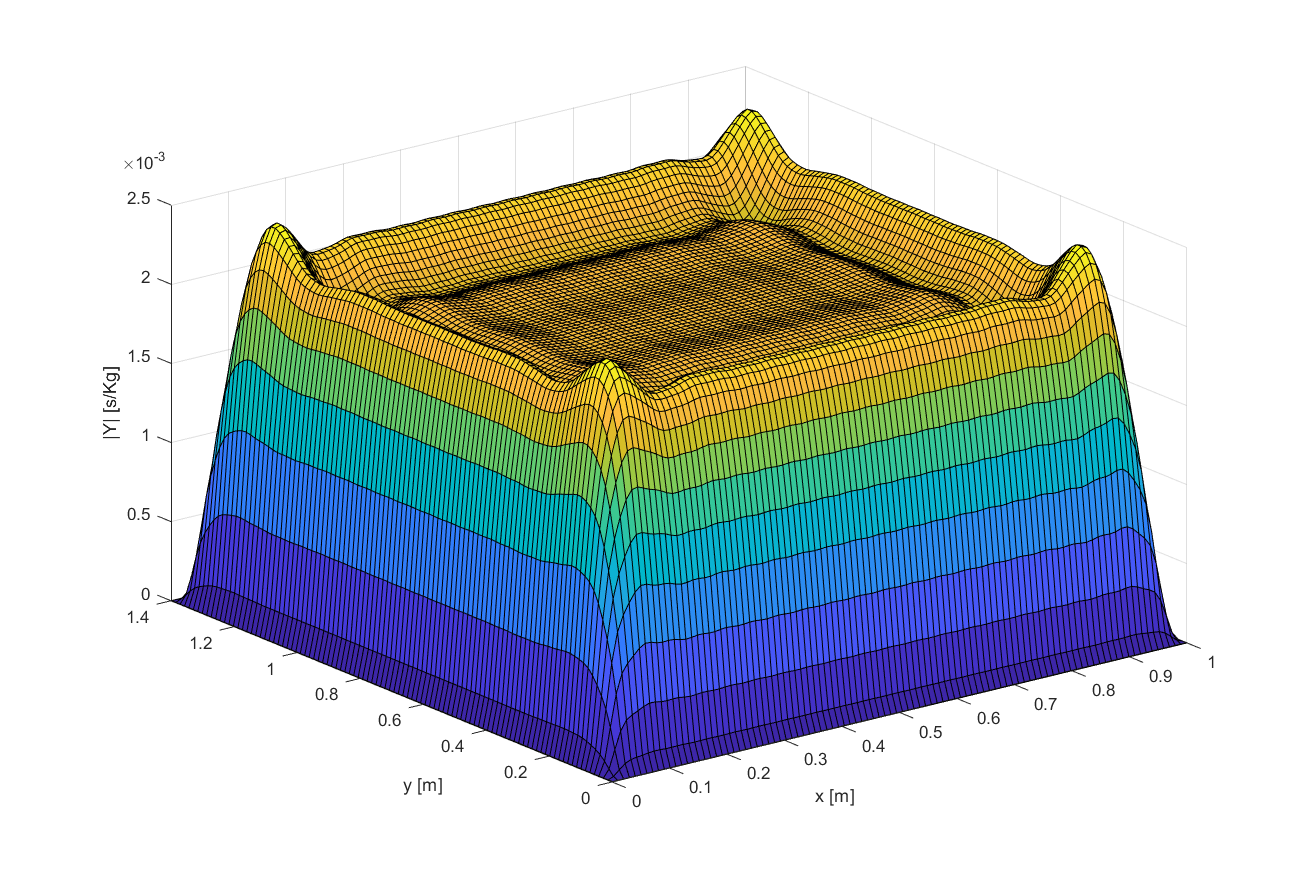
\includegraphics[width=0.7\textwidth]{admittance.png}
	\caption{Graph of the absolute value of the input admittance of the plate at $f_0 = \SI{130.8}{\hertz}$.}
	\label{fig:adm}
\end{figure}

\section{Doublet of strings mounted to the plate}

Following the treatment presented in \cite{chker}, we obtain that the eigenfrequencies of a pair of strings coupled to a soundboard can be written as a function of the detuning $\epsilon$:

$$ \omega_{\pm} + j \frac{1}{\tau_{\pm}} = \chi + \epsilon \pm \sqrt{\chi^2 + \epsilon^2}  $$
where $\chi$ is defined by $Y_B = \frac{\pi }{j Z_0}\chi$ and $Z_0$ is the characteristic impedance of the first string. When placing the bridge at one of the admittance maxima, we get $\chi = -0.0014 + j 0.0017$. With this value we can plot $\omega_{\pm}$ and $\tau_{\pm}$ as functions of $\epsilon$, as seen in Fig. \ref{fig:doub}. As expected, the decay time of one string diverges when $\epsilon$ goes to zero while the other only decreases slightly.

\begin{figure}[h]
	\centering
	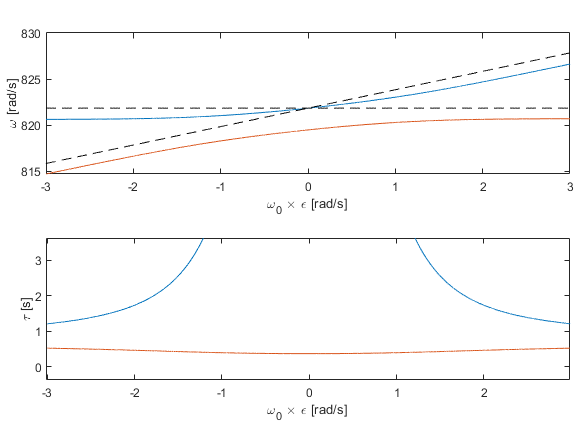
\includegraphics[width=0.8\textwidth]{doublet.png}
	\caption{Eigenfrequencies and decay times of the string doublet when coupled to the plate, as a function of the detuning $\epsilon$.}
	\label{fig:doub}
\end{figure}

\printbibliography

\appendix
\newpage
\section{COMSOL Simulations}


\begin{figure}[h]
	\centering
	\begin{subfigure}[b]{0.31\linewidth}
		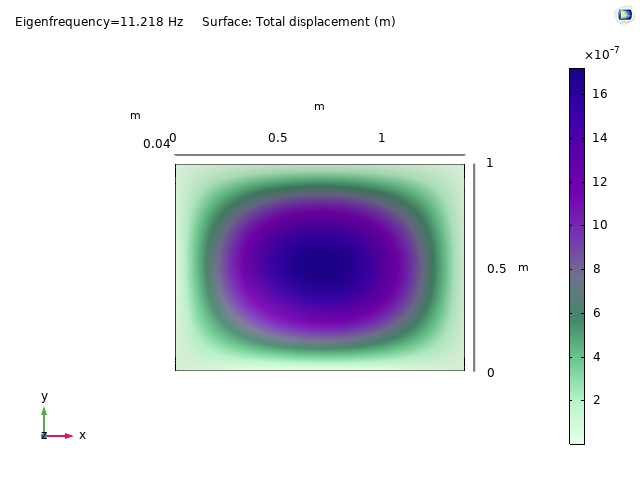
\includegraphics[width=0.9\linewidth]{comsol/1ss.png}
		\caption*{\SI{11.218}{\hertz}}
	\end{subfigure}
	~
	\begin{subfigure}[b]{0.31\linewidth}
		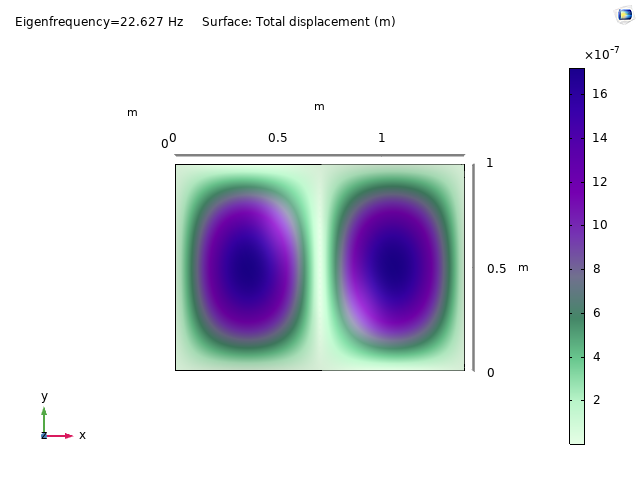
\includegraphics[width=0.9\linewidth]{comsol/2ss.png}
		\caption*{\SI{22.627}{\hertz}}
	\end{subfigure}
	~
	\begin{subfigure}[b]{0.31\linewidth}
		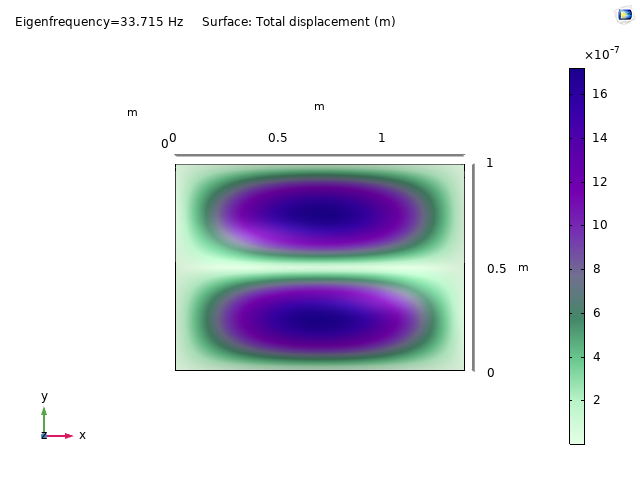
\includegraphics[width=0.9\linewidth]{comsol/3ss.png}
		\caption*{\SI{33.715}{\hertz}}
	\end{subfigure}

	\begin{subfigure}[b]{0.31\linewidth}
		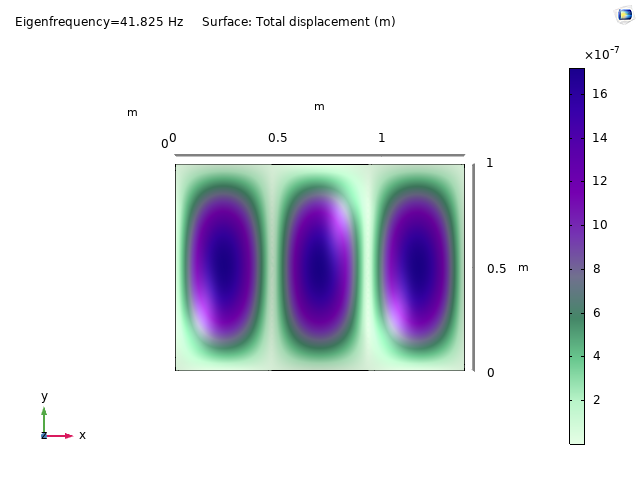
\includegraphics[width=0.9\linewidth]{comsol/4ss.png}
		\caption*{\SI{41.825}{\hertz}}
	\end{subfigure}
	~
	\begin{subfigure}[b]{0.31\linewidth}
		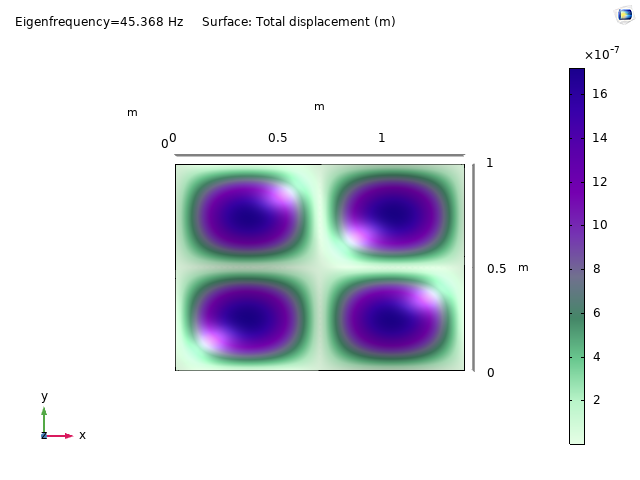
\includegraphics[width=0.9\linewidth]{comsol/5ss.png}
		\caption*{\SI{45.368}{\hertz}}
	\end{subfigure}
	\caption{Eigenshapes for the \textbf{supported edges} case as computed with COMSOL.}
	\label{fig:ss_com}
\end{figure}

\begin{figure}[h]
	\centering
	\begin{subfigure}[b]{0.31\linewidth}
		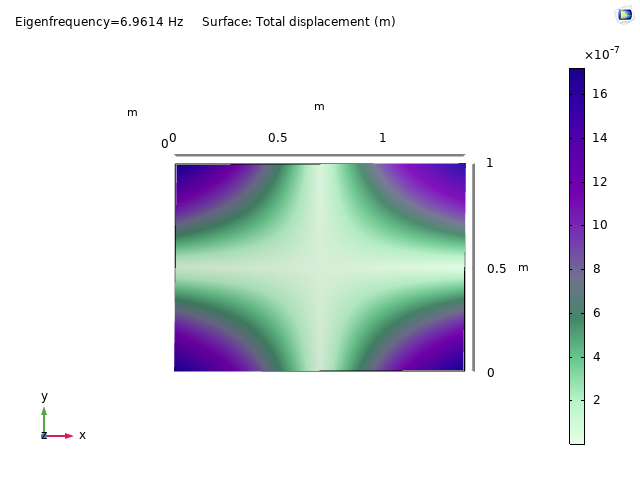
\includegraphics[width=0.9\linewidth]{comsol/1f.png}
		\caption*{\SI{6.9614}{\hertz}}
	\end{subfigure}
	~
	\begin{subfigure}[b]{0.31\linewidth}
		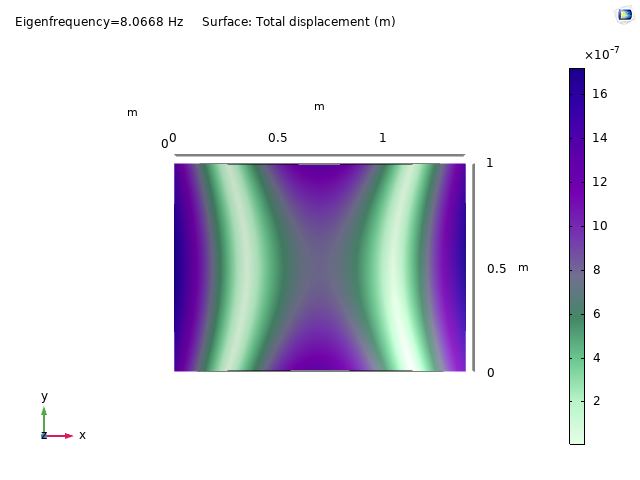
\includegraphics[width=0.9\linewidth]{comsol/2f.png}
		\caption*{\SI{8.0668}{\hertz}}
	\end{subfigure}
	~
	\begin{subfigure}[b]{0.31\linewidth}
		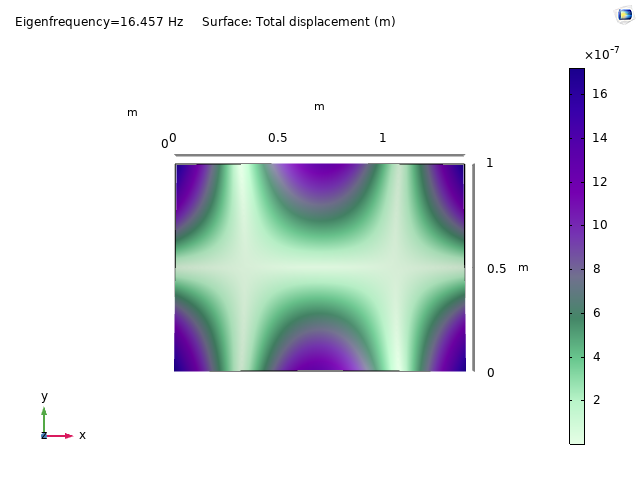
\includegraphics[width=0.9\linewidth]{comsol/3f.png}
		\caption*{\SI{16.457}{\hertz}}
	\end{subfigure}
	
	\begin{subfigure}[b]{0.31\linewidth}
		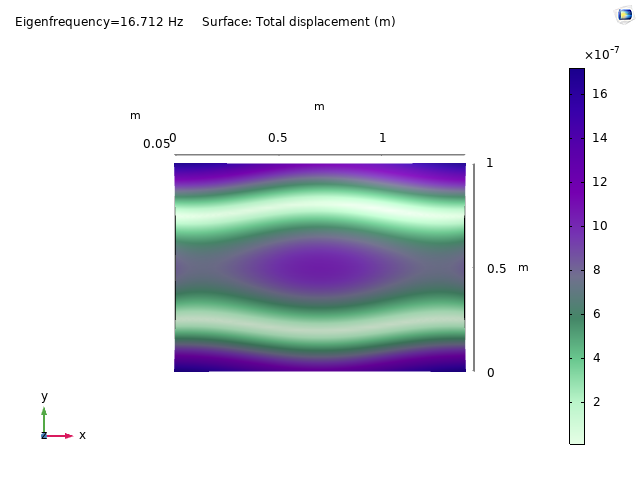
\includegraphics[width=0.9\linewidth]{comsol/4f.png}
		\caption*{\SI{16.712}{\hertz}}
	\end{subfigure}
	~
	\begin{subfigure}[b]{0.31\linewidth}
		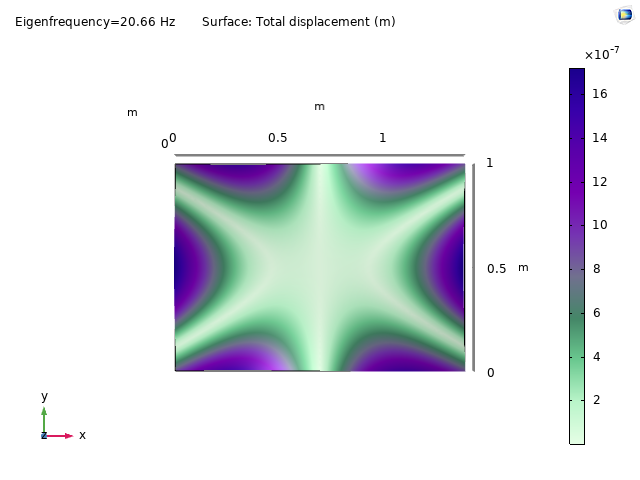
\includegraphics[width=0.9\linewidth]{comsol/5f.png}
		\caption*{\SI{20.66}{\hertz}}
	\end{subfigure}
	\caption{Eigenshapes for the \textbf{free edges} case as computed with COMSOL.}
	\label{fig:f_com}
\end{figure}

\begin{figure}[h]
	\centering
	\begin{subfigure}[b]{0.31\linewidth}
		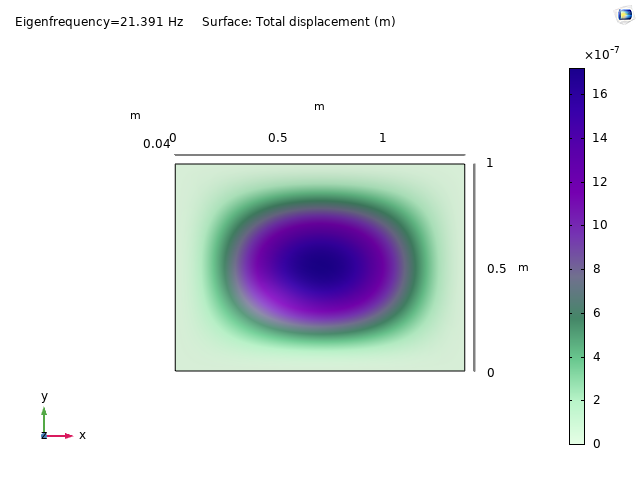
\includegraphics[width=0.9\linewidth]{comsol/1c.png}
		\caption*{\SI{21.391}{\hertz}}
	\end{subfigure}
	~
	\begin{subfigure}[b]{0.31\linewidth}
		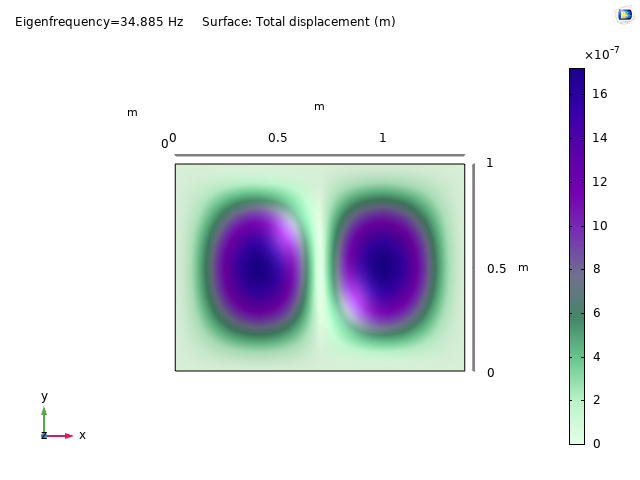
\includegraphics[width=0.9\linewidth]{comsol/2c.png}
		\caption*{\SI{34.885}{\hertz}}
	\end{subfigure}
	~
	\begin{subfigure}[b]{0.31\linewidth}
		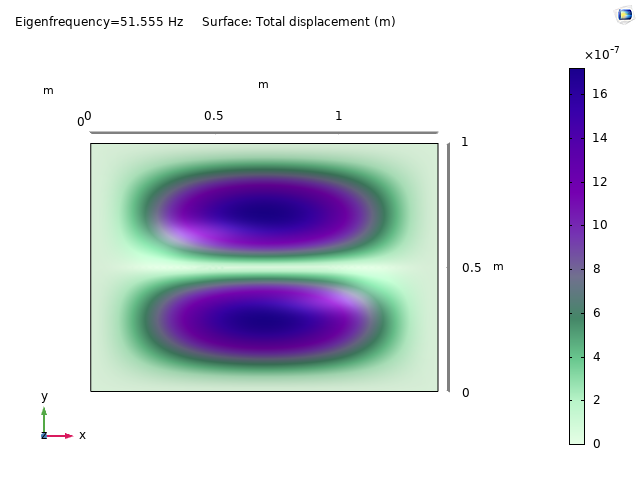
\includegraphics[width=0.9\linewidth]{comsol/3c.png}
		\caption*{\SI{51.555}{\hertz}}
	\end{subfigure}
	
	\begin{subfigure}[b]{0.31\linewidth}
		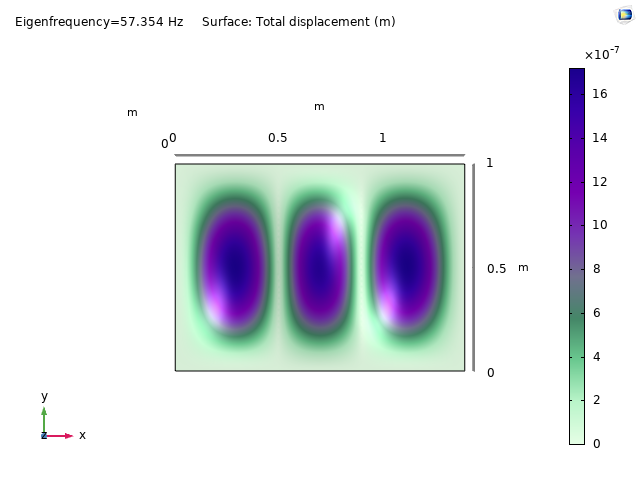
\includegraphics[width=0.9\linewidth]{comsol/4c.png}
		\caption*{\SI{57.354}{\hertz}}
	\end{subfigure}
	~
	\begin{subfigure}[b]{0.31\linewidth}
		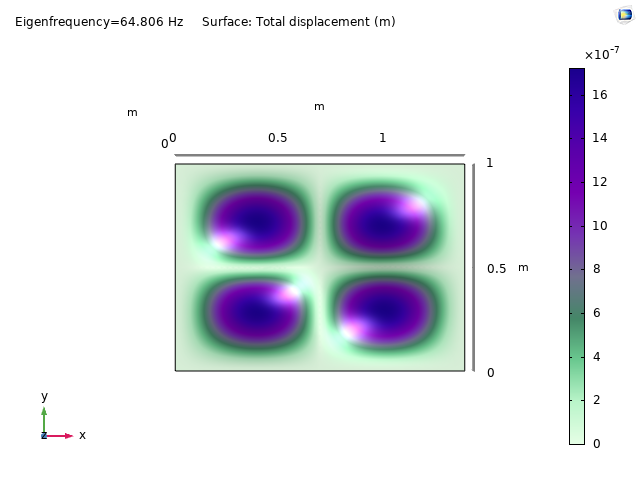
\includegraphics[width=0.9\linewidth]{comsol/5c.png}
		\caption*{\SI{64.806}{\hertz}}
	\end{subfigure}
	\caption{Eigenshapes for the \textbf{clamped edges} case as computed with COMSOL.}
	\label{fig:c_com}
\end{figure}



\end{document}